\documentclass[twoside]{article}

\usepackage[sc]{mathpazo} % Use the Palatino font
\usepackage[T1]{fontenc} % Use 8-bit encoding that has 256 glyphs
\linespread{1.05} % Line spacing - Palatino needs more space between lines
\usepackage{microtype} % Slightly tweak font spacing for aesthetics

\usepackage[hmarginratio=1:1,top=32mm,columnsep=20pt]{geometry} % Document margins
\usepackage{multicol} % Used for the two-column layout of the document
\usepackage[hang, small,labelfont=bf,up,textfont=it,up]{caption} % Custom captions under/above floats in tables or figures
\usepackage{booktabs} % Horizontal rules in tables
\usepackage{float} % Required for tables and figures in the multi-column environment - they need to be placed in specific locations with the [H] (e.g. \begin{table}[H])
\usepackage{hyperref} % For hyperlinks in the PDF

\usepackage{lettrine} % The lettrine is the first enlarged letter at the beginning of the text
\usepackage{paralist} % Used for the compactitem environment which makes bullet points with less space between them

\usepackage{graphicx}
\usepackage{caption}
\usepackage{subcaption}

\usepackage{abstract} % Allows abstract customization
\renewcommand{\abstractnamefont}{\normalfont\bfseries} % Set the "Abstract" text to bold
\renewcommand{\abstracttextfont}{\normalfont\small\itshape} % Set the abstract itself to small italic text

\usepackage{titlesec} % Allows customization of titles
\renewcommand\thesection{\Roman{section}} % Roman numerals for the sections
\renewcommand\thesubsection{\Roman{subsection}} % Roman numerals for subsections
\titleformat{\section}[block]{\large\scshape\centering}{\thesection.}{1em}{} % Change the look of the section titles
\titleformat{\subsection}[block]{\large}{\thesubsection.}{1em}{} % Change the look of the section titles

\usepackage{fancyhdr} % Headers and footers
\pagestyle{fancy} % All pages have headers and footers
\fancyhead{} % Blank out the default header
\fancyfoot{} % Blank out the default footer
\fancyhead[C]{EECS 584 $\bullet$ October 2nd, 2014 $\bullet$ Barzan Mozafari} % Custom header text
\fancyfoot[RO,LE]{\thepage} % Custom footer text

%----------------------------------------------------------------------------------------
%	TITLE SECTION
%----------------------------------------------------------------------------------------

\title{\vspace{-15mm}\fontsize{24pt}{10pt}\selectfont\textbf{Extending BlinkDB With Fundamental Analytical Operations: Linear Regression}} % Article title

\author{
\large
\textsc{Nathan Harada, Julian Katz-Samuels}\\[2mm] % Your name
\normalsize University of Michigan \\ % Your institution
\normalsize $\{$nharada, jkatzsam$\}$@umich.edu
\vspace{-5mm}
}
\date{}

%----------------------------------------------------------------------------------------

\begin{document}

\maketitle % Insert title

\thispagestyle{fancy} % All pages have headers and footers

%----------------------------------------------------------------------------------------
%	RESULTS
%----------------------------------------------------------------------------------------
\section{Evaluation}
\subsection{Evaluation Datasets}
We evaluated our extensions to BlinkDB via a generated synthetic benchmark as well as the bike sharing dataset from the University of California Irvine Machine Learning Repository (UCI-ML), a collection of standard and well studied datasets available to the research community. The synthetic dataset was generated in Matlab via the equation $y=X\beta + \varepsilon$, where $X\sim\mathcal{N}\left(0,1\right)$ and $\varepsilon$ represents additive white Gaussian noise with a signal to noise ratio of 0dB. We fixed the values fo $\beta$ to $[1,-2,3]$.

\subsection{Evaluation Setting}
Experiments were perfomed on a single-node system, configured with 8 GB of RAM, 6 CPU cores (2.67 GHz), 1TB of disk running Ubuntu 14.04. BlinkDB alpha release 0.2 was used as the base software, along with Scala 2.10 and Spark SQL 1.1.0. To evaluate the correctness of the implemented algorithms, we used IBM SPSS Statistics 21.

\subsection{Synthetic Dataset}
The full synthetic dataset consists of 10 million rows of data, each consisting of independent variables $x,y,z$ and dependent variable $u$. The dataset was sampled with various sampling probabilities, with the true sample sizes listed below:

\begin{center}
    \begin{tabular}{| l | l |}
	\hline
	Sampling Probability & Resulting Sample Size \\
	\hline
	0.0001 & 999 \\
	0.0003 & 3000 \\
	0.0008 & 8112 \\
	0.001 & 9950 \\
	0.003 & 29967 \\
	0.01 & 100390 \\
	0.1 & 999682 \\
	Full & 10000000 \\
	\hline
    \end{tabular}
\end{center}

To test the accuracy of our system, we first compared the true coefficient values with the estimated coefficients. The mean squared error between $\beta$ and $\hat \beta$ was calculated for each of the sample sizes. We show that as the sample size increases, the values of $\hat \beta$ asymptotically approach the true values of $\beta$. Error rate drops quickly as sample size increases, with a fraction of a percentage of the original dataset presenting nearly accurate results. We repeated the experiment for the calculated confidence intervals on each sample. Again, as sample size increases, the confidence interval width shinks, approaching zero as the sample size grows large.

\begin{figure}[htb]
        \centering
        \begin{subfigure}{0.45\textwidth}
                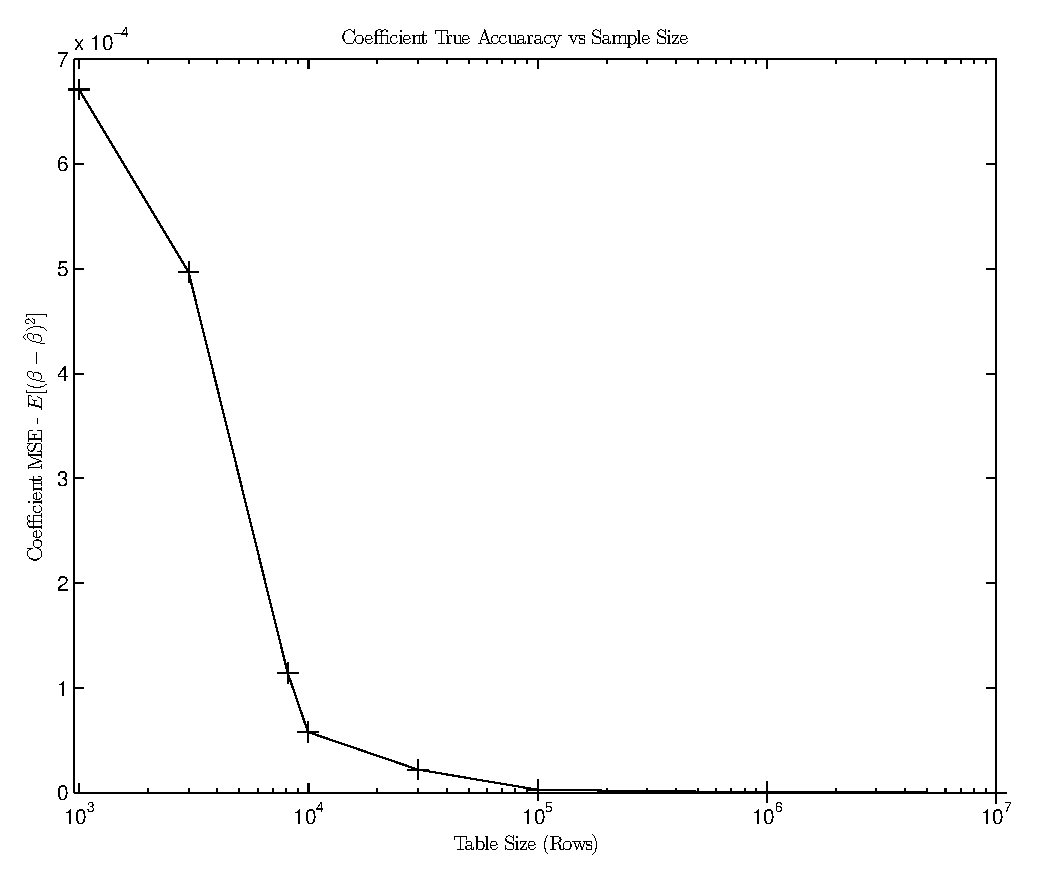
\includegraphics[width=\textwidth]{accuracy}
                \caption{Coefficient accuracy vs Sample Size (log scale)}
                \label{fig:accuracy}
        \end{subfigure}
        \begin{subfigure}{0.45\textwidth}
                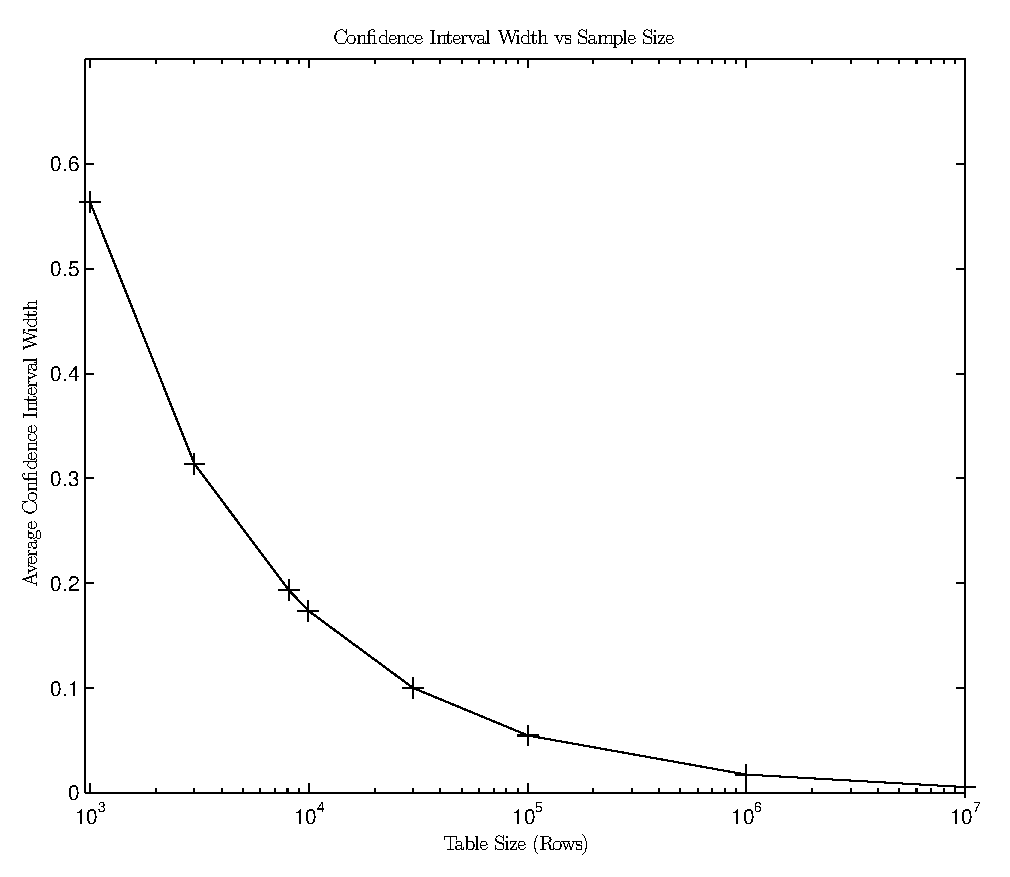
\includegraphics[width=\textwidth]{confidence}
                \caption{Confidence Interval Width vs Sample Size (log scale)}
                \label{fig:confidence}
        \end{subfigure}
\end{figure}

We additionally recorded and plotted the runtime for each query. Runtime appears to scale linearly with table size, meaning that a user who wishes to perform an approximate linear regression can easily trade off error for time to achieve reasonable confidence intervals within an interactive time frame.

\begin{figure}[htb]
        \centering
        \begin{subfigure}{0.45\textwidth}
                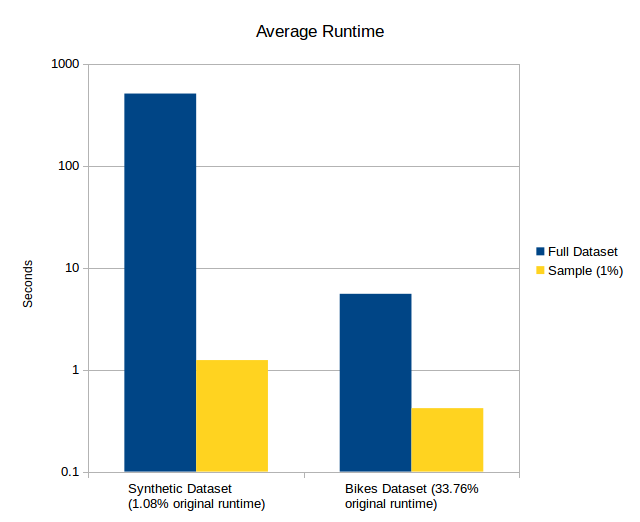
\includegraphics[width=\textwidth]{synthvreal}
                \caption{Query Runtime on a synthetic and real world dataset}
                \label{fig:synthvreal}
        \end{subfigure}
        \begin{subfigure}{0.45\textwidth}
                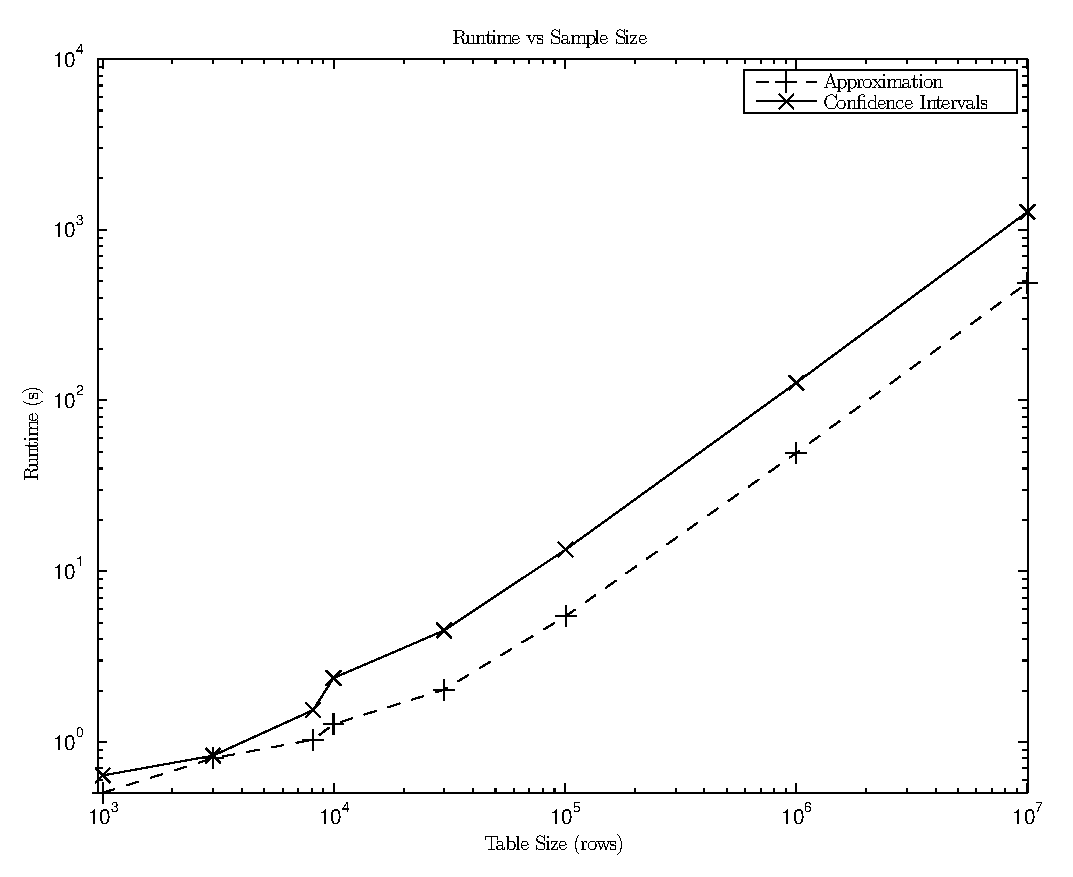
\includegraphics[width=\textwidth]{runtime}
                \caption{Query Runtime (log scale) vs Sample Size (log scale)}
                \label{fig:runtime}
        \end{subfigure}
\end{figure}

\subsection{Bike Sharing Dataset}
The bike sharing dataset contains the hourly and daily counts of bike rentals for Washington DC's bikeshare program, along with relevant weather data such as humidity and windspeed. We evaluated the runtime performance of our system on this dataset, and compared it to the performance of our larger synthetic dataset. While both datasets achieved a significant increase in speed, the real world dataset saw less of an improvement compared to our synthetic data. We suspect this is because, while we only chose a few independent variables to regress, the full dataset contains many more columns. This additional overhead likely resulted in additional disk overhead that limited our performance gains.

%----------------------------------------------------------------------------------------
%	REFERENCE LIST
%----------------------------------------------------------------------------------------

\begin{thebibliography}{99} % Bibliography - this is intentionally simple in this template

\bibitem[1]{Agarwal:2010}
Agarwal, Sameer, et al. "BlinkDB: queries with bounded errors and bounded response times on very large data." Proceedings of the 8th ACM European Conference on Computer Systems. ACM, 2013.

\bibitem[2]{Brown:2010}
Brown, Paul G. "Overview of SciDB: large scale array storage, processing and analysis." Proceedings of the 2010 ACM SIGMOD International Conference on Management of data. ACM, 2010.
 
\end{thebibliography}

%----------------------------------------------------------------------------------------

\end{document}